

%%%%%%%%%%%%%%%%%%%%%%%%%%%%%%%%%%%%%%%%%%%%%%%%%%%%%%%%%%%%%%%%%%%%%%%%
%    INSTITUTE OF PHYSICS PUBLISHING                                   %
%                                                                      %
%   `Preparing an article for publication in an Institute of Physics   %
%    Publishing journal using LaTeX'                                   %
%                                                                      %
%    LaTeX source code `ioplau2e.tex' used to generate `author         %
%    guidelines', the documentation explaining and demonstrating use   %
%    of the Institute of Physics Publishing LaTeX preprint files       %
%    `iopart.cls, iopart12.clo and iopart10.clo'.                      %
%                                                                      %
%    `ioplau2e.tex' itself uses LaTeX with `iopart.cls'                %
%                                                                      %
%%%%%%%%%%%%%%%%%%%%%%%%%%%%%%%%%%
%
%
% First we have a character check
%
% ! exclamation mark    " double quote  
% # hash                ` opening quote (grave)
% & ampersand           ' closing quote (acute)
% $ dollar              % percent       
% ( open parenthesis    ) close paren.  
% - hyphen              = equals sign
% | vertical bar        ~ tilde         
% @ at sign             _ underscore
% { open curly brace    } close curly   
% [ open square         ] close square bracket
% + plus sign           ; semi-colon    
% * asterisk            : colon
% < open angle bracket  > close angle   
% , comma               . full stop
% ? question mark       / forward slash 
% \ backslash           ^ circumflex
%
% ABCDEFGHIJKLMNOPQRSTUVWXYZ 
% abcdefghijklmnopqrstuvwxyz 
% 1234567890
%
%%%%%%%%%%%%%%%%%%%%%%%%%%%%%%%%%%%%%%%%%%%%%%%%%%%%%%%%%%%%%%%%%%%
%
 \documentclass[twocolumn,11pt,a4paper]{article}		%<-use this for checking equation length
% \documentclass[12pt]{iopart} 

%<-comment out this for checking equations (author list too)
% \usepackage{iopams,setstack} 
%<-comment out this for checking equations
\usepackage{graphicx}
\usepackage{algorithm, algorithmicx, algpseudocode} 
\usepackage{color} 
%This is to decrease the space in subfigure command
\usepackage[tight,scriptsize]{subfigure}
\makeatletter
\renewcommand{\subfigtopskip}{1\p@}
\renewcommand{\subfigcapskip}{0\p@}
\renewcommand{\subfigcaptopadj}{1\p@}
\renewcommand{\subfigbottomskip}{1\p@}
\renewcommand{\subfiglabelskip}{0.05em plus 0.02em minus 0.01em}
\makeatother
% \usepackage{pstool}
\renewcommand{\subcapsize}{\small}
 \usepackage{anysize}							%<-use this for checking equation length
 \marginsize{1.7cm}{1.5cm}{0.3cm}{0.8cm}			%<-use this for checking equation length
 \setlength{\columnsep}{0.5cm}					%<-use this for checking equation length
 \usepackage{amsmath}
\usepackage{amssymb,amsfonts} 			%<-use this for checking equation length
\newcommand{\todo}[1]{\textsf{\emph{\textbf{\textcolor{blue}{#1}}}}} 
\newcommand{\wtf}[1]{\textsf{\emph{\textbf{\textcolor{red}{#1}}}}} 
\newcommand{\omg}[1]{\textsf{\emph{\textbf{\textcolor{green}{#1}}}}} \begin{document}

% \begin{document}

\title[State and Parameter Estimation for Spatio-Temporal Neural Fields]{State and Parameter Estimation for Spatio-Temporal Neural Fields}

\author{Dean R. Freestone$^1$, Parham Aram$^2$, Michael Dewar$^3$, Kenneth Scerri$^4$, David B. Grayden$^1$, and Visakan Kadirkamanathan$^2$}

% \address{$^1$ Department of Electrical and Electronic Engineering, University of Melbourne, Melbourne, Vic, 3010 Australia} \address{$^2$ Department of Automatic Control and Systems Engineering, University of Sheffield, Mappin Street, Sheffield, S1 3JD, UK} \address{$^3$ Department of Applied Physics and Applied Mathematics, Columbia University, US} \address{$^4$ Ken's} \ead{dfreestone@bionicear.org} 
\begin{abstract}
	Will do the abstract towards the end. 
\end{abstract}

%Uncomment for PACS numbers title message
%\pacs{00.00, 20.00, 42.10}
% Keywords required only for MST, PB, PMB, PM, JOA, JOB? 
%\vspace{2pc}
%\noindent{\it Keywords}: Article preparation, IOP journals
% Uncomment for Submitted to journal title message
%\submitto{\JPA}
% Comment out if separate title page not required
\maketitle

\section{Introduction} This paper presents a theoretical framework for generating macroscopic neural field mathematical models from patient specific data. There has been much interest in generating physiologically plausible neural field models to study brain dynamics at the meso/macroscopic scale. While our understanding of the function of neurons is well developed, the overall behaviour of the brain's meso and macro-scale dynamics remains largely a theoretical. Understanding the brain at this level is extremely important since this is the scale where pathologies such as epilepsy, Parkinson's disease and schizophrenia are manifested. Mathematical neural field models provide insights into the underlying physics and dynamics of electroencephalography (EEG) and magnetoencephalography (MEG) (see \cite{Deco2008,David2003} for recent reviews). These models have demonstrated possible mechanisms for the genesis of neural rhythms (such as the alpha and gamma rhythms) \cite{Liley1999,RENNIE2000}, epileptic seizure generation \cite{DaSilva2003,Suffczynski2004,Wendling2005} and insights into other pathologies \cite{Moran2008,Schiff2009} that would be difficult to gain from experimental data alone. 

Unfortunately, the use of these models in the clinic has been limited, since they are constructed for ``general'' brain dynamics whereas pathologies almost always have unique underlying patient specific causes. Patient specific data from EEG is readily available in the clinical setting, suggesting an opportunity to make the patient-specific link to models of cortical dynamics. However the meso/macroscopic neural dynamic state is not directly observable in EEG data, making predictions of the underlying physiology inherently difficult.

For models to be clinically viable they must be patient specific. A possible approach to achieve this would be to fit a general neural field model, like the Wilson and Cohen (WC) \cite{Wilson1973} model or a neural mass model like the Jansen and Ritt model \cite{Jansen1995}, to patient specific EEG data. Fitting the neural models to individuals is a highly non-trivial task, and until very recently this has not been reported in the literature. 

An estimation framework for neural field models known as dynamical causal modelling (DCM) \cite{David2003,David2006} has recently been proposed for studying evoked potential dynamics. Via a Bayesian inference scheme, DCM estimates the long range connectivity structure between the specific isolated brain regions that best explains a given data set under the Jansen and Ritt equations. Another recent publication describing a parameter estimation method with a neural field model used an unscented Kalman filter with the WC neural field equations \cite{schiff2008kalman}. This work takes a system theoretic approach to the neural estimation problem, successfully demonstrating it is possible to perform state estimation of modified WC equations. This marks the first step in what has the potential to revolutionise the treatment of many neurological diseases where therapeutic electrical stimulation is viable.

%Currently available epileptic seizure  control devices (i.e., the vagal nerve stimulator) are implemented in an ``open loop". That is, the therapeutic electrical stimulation waveforms are adjusted for each patient by trial and error, disregarding the patient's neuro-dynamics and information about their particular pathologies. Given access to an accurate model, the application of optimal control theory in these circumstances would allow for robust therapeutic stimulations.

This paper extends the work of Schiff and Sauer~\cite{schiff2008kalman} by establishing a framework for estimating the state of the WC equations for higher order systems via a systematic model reduction procedure. In addition, a method is presented for estimating the connectivity structure and the synaptic time constant. Until now, estimation of local intracortical connectivity structure has not been attempted. Recently, it has been shown that it is possible to estimate local coupling of spatiotemporal systems using techniques from control systems theory and machine learning \cite{Dewar2009}. The key development in that work was to represent the spatiotemporal system as a standard state-space model with an order independent of the number of observations (recording electrodes in this case). In addition, the appropriate model selection tools have been developed \cite{Scerri2009} allowing for the application of the technique to neural fields. 

Modelling the neural dynamics within this framework has the distinct advantage over the more standard multivariate auto-regressive (AR) models: that the number of parameters to define the spatial connectivity is considerably smaller than the number of AR coefficients typically required to achieve the required model complexity. 

In this paper, we demonstrate for the first time how intracortical connectivity can be inferred from data, based on a variant of the Wilson and Cowan neural field model \cite{Wilson1973}. This work provides a fundamental link between the theoretical advances in neural field modelling and patient specific data.

The paper proceeds by first deriving the continuum neural field equations in Section~\ref{NeuralModelSection}. Next, a reduced finite dimensional neural field model is derived. The model is reduced by approximating the neural field using a set of continuous basis functions, weighted by a finite dimensional state vector. Section~\ref{SpectralAnalysisSection} establishes conditions using spatial frequency analysis for both sensor and basis function spacing and geometry, such that the dominant dynamics of the neural field can be represented by the reduced model. Following this, the state and parameter estimation procedure is described in Section~\ref{StateAndParameterEstimationSection}. The results for the spatial frequency analysis and parameter estimation are then presented in Section~\ref{ResultsSection}. The implications and limitations of this framework are discussed in Section~\ref{DiscussionSection} along with planned future developments. Finally, we provide concluding remarks in Section~\ref{ConclusionSection}.

\section{Neural Field Model}\label{NeuralModelSection} In this section, we describe a variant of the WC or Amari style neural field model \cite{Wilson1973,Amari1977} that was used to create our intracortical connectivity estimator. Neural field models relate mean firing rates of pre-synaptic neural populations to mean post-synaptic membrane potentials. They are popular due to being parsimonious yet having a strong link with the underlying physiology. Each neural population represents a functional cortical processing unit, such as a column. The columnar organisation of the cortex is continuous, where pyramidal cells are members of many columns. In general, cortical structure can be modelled in a physiologically plausible manner as being locally homogeneous (in short range intracortical connectivity) and heterogeneous (in long range cortico-cortical and corticothalamic connectivity)~\cite{Jirsa2009,Qubbaj2007}. Locally, each column is thought be connected via symmetric short range local excitation, with surround inhibition \cite{Braitenberg1998}. For example, this structural organisation is most studied in the visual system, where the surrounding inhibition effectively tunes a cortical column to a particular receptive visual field~\cite{Sullivan2006}. Neural field models are descriptive of a range of neurodynamics of the cortex such as evoked potentials, visual hallucinations, and epileptic behaviour~\cite{David2003,Bressloff2001,Breakspear2006}. 
Field models are also capable of generating complex patterns of activity such as Turing patterns, spirals, and traveling oscillations~\cite{Amari1977,Coombes2005,Coombes2007}.

\subsection{Derivation of the Integro-difference Equation Representation}

The model relates the average number of action potentials $g(\mathbf{r},t)$ arriving at position $\mathbf{r}$ to the local post synaptic membrane voltage $v(\mathbf{r},t)$. The post-synaptic potentials generated at a neuronal population at location $\mathbf{r}$ by action potentials arriving from all other connected populations at locations $\mathbf{r}'$ can be described by 
\begin{equation}
	\label{SpikesToPotential} v\left( {\mathbf{r},t} \right) = \int_{ - \infty }^t {h\left( {t - t'} \right)g\left( {\mathbf{r},t'} \right)dt'}. 
\end{equation}
The post-synaptic response kernel $h(t)$ is described by 
\begin{equation}
	\label{SynapticRespKernel} h(t) = \eta(t)\exp{\left(-\zeta t\right)}. 
\end{equation}
where $\zeta=\tau^{-1}$ and $\tau$ is the synaptic time constant and $\eta(t)$ is the Heaviside step function. Nonlocal interactions between cortical populations are described by 
\begin{equation}
	\label{RateBasedInteractions} g\left( \mathbf{r},t \right) = \int_\Omega {w\left( \mathbf{r},\mathbf{r}' \right)f\left( v\left( \mathbf{r}',t \right) \right)d\mathbf{r}'}, 
\end{equation}
where $f(\cdot)$ is the firing rate function, $w(\cdot)$ is the spatial connectivity kernel, and $\Omega$ is the spatial domain, representing a cortical sheet or surface. The connectivity kernel is typically a ``Mexican hat'' function which describes strong local activation, weak mid-range repression and weak long-range activation. The exact shape of this kernel is assumed to vary across patients, and hence needs to be inferred from data. 

The firing rate of the presynaptic neurons is related to the postsynaptic membrane potential by the sigmoidal activation function 
\begin{equation}
	\label{ActivationFunction} f\left( v\left( \mathbf{r}', t \right) \right) = \frac{f_{max}\left(\mathbf{r}\right)}{1 + \exp \left( \varsigma \left( v_0\left( \mathbf{r} \right) - v\left(\mathbf{r}',t\right) \right) \right)}. 
\end{equation}
The parameters $f_{max}$ and $v_0$ describe the maximum firing rate and firing threshold of the neural populations. The parameter $\varsigma$ governs the slope of the sigmoid. By substituting equation~\ref{RateBasedInteractions} into \ref{SpikesToPotential} we get the spatiotemporal model 
\begin{eqnarray}
	\label{FullDoubleIntModel} v\left(\mathbf{r},t\right) &=&  \int_{-\infty}^t h\left(t - t'\right) \\
	&\times&\int_\Omega w\left(\mathbf{r},\mathbf{r}'\right) f\left( v\left( \mathbf{r}',t \right)\right)d\mathbf{r}'dt'. \nonumber
\end{eqnarray}
To arrive at the final form of the model we shall state the synaptic response kernel as a Green's function 
\begin{equation}
	\label{GreensFuncDef} Dh\left( t \right) = \delta \left( t \right), 
\end{equation}
where $D=\frac{d}{dt} + \zeta$ is a temporal differential operator and $\delta(t)$ is the Dirac-delta function giving 
\begin{eqnarray}
	\label{FinalFormContinuous} \frac{dv\left( \mathbf{r},t \right)}{dt} &+& \zeta v\left( \mathbf{r},t \right) = \\
	&&\int_\Omega {w\left( \mathbf{r},\mathbf{r}' \right)f\left( {v\left( \mathbf{r}',t \right)} \right)d\mathbf{r}'}. \nonumber
\end{eqnarray}
To arrive at the integro-difference equation (IDE) form of the model we discretise time using a first-order Euler method (see Appendix~\ref{Time Discretization}) giving 
\begin{eqnarray}
	\label{DiscreteTimeModel} v_{t+1}\left(\mathbf{r}\right) &=& \xi v_t\left(\mathbf{r}\right) + T_s \int_\Omega { w\left(\mathbf{r}-\mathbf{r}'\right) f\left(v_t\left(\mathbf{r}'\right)\right) d\mathbf{r}'} \nonumber\\ 
	&+& e_t\left(\mathbf{r}\right), 
\end{eqnarray}
where $T_s$ is the time step, $\xi = 1-\zeta T_s$ and $e_t(\mathbf{r})$ is i.i.d. such that $e_t\sim\mathcal{GP}(\mathbf 0,\gamma(\mathbf{s}-\mathbf{r}))$. This term was added to account for uncertainty in the model. To generate iEEG/LFP data we used the output function 
\begin{equation}
	\mathbf{y}_t = \int_{\Omega}{m\left(\mathbf{r}_n-\mathbf{r}'\right)v_t\left(\mathbf{r}'\right)d\mathbf{r}'} + \boldsymbol{\varepsilon}_t, 
\end{equation}
where $\mathbf{r}_n$ defines the location of the sensors in the field where $n=1,...,N$ indexes the sensors and $\boldsymbol{\varepsilon}_t \sim \mathcal{N}\left(0,\Sigma_{\varepsilon}\right)$. The output kernel $m(\mathbf{r}-\mathbf{r}')$ governs the geometry of pick-up range of sensors where 
\begin{equation}
	m\left(\mathbf{r}-\mathbf{r}'\right) = \exp{\left(-\frac{(\mathbf{r}-\mathbf{r}')^\top(\mathbf{r}-\mathbf{r}')}{\sigma_m^2}\right)}. 
\end{equation}

\subsection{Derivation of Finite Dimensional State-Space Model} 
In order to implement standard estimation techniques we use a decomposition of the field using a set of Gaussian basis functions defined by
\begin{equation}\label{eq:FieldBasisFunction}
	\phi\left(\mathbf{r}-\mathbf{r}'\right) =
\exp{\left(-\frac{(\mathbf{r}-\mathbf{r}')^\top(\mathbf{r}-\mathbf{r}')}{\sigma_{\phi}^2}\right)}. 
\end{equation}
 Decomposition allows a continuous field to be represented by a finite dimensional state vector. This facilitates application of standard nonlinear state estimation methods such as the unscented Kalman filter. The field decomposition is described by 
\begin{equation}
	\label{DefFieldDecomp} v_t\left(\mathbf{r}\right) \approx \boldsymbol{\phi}^{\top}\left(\mathbf{r}\right) \mathbf{x}_t, 
\end{equation}
where $\mathbf{\boldsymbol{\phi}}(\mathbf{r})$ is a vector of Gaussian basis functions that are scaled by the state vector, $\mathbf{x}_t$. The width and positioning of the basis function can be determined by spectral analysis explain in detail in Section~\ref{SpectralAnalysisSection}. The connectivity kernel can also be considered a decomposition into a set of basis functions in 
\begin{equation}\label{DefKernelDecomp}
	 w\left(\mathbf{r}-\mathbf{r}'\right) =\boldsymbol{\psi}^\top\left(\mathbf{r}-\mathbf{r}'\right) \boldsymbol{\theta}.
\end{equation}
We will assume we know the parametric form of the connectivity basis functions, where the parameter $\boldsymbol{\theta}$ is unknown. Each connectivity basis function can, individually, be considered a layer in the Wilson and Cowan model, representing short range excitation, surround inhibition and mid-range excitation. Making substitutions of equations~\ref{DefFieldDecomp} and~\ref{DefKernelDecomp} into~\ref{DiscreteTimeModel} we get 
\begin{eqnarray}
	\label{reduced continuous model}\boldsymbol{\phi}^{\top}(\mathbf{r})\mathbf{x}_{t+1}&=& T_s\int_\Omega{f(\boldsymbol{\phi}^{\top}(\mathbf{r}')\mathbf{x}_t )\boldsymbol{\psi}^{\top}(\mathbf{r}-\mathbf{r}')d\mathbf{r}'}\boldsymbol{\theta}\nonumber \\ 
	&-& \xi\boldsymbol{\phi}^{\top}(\mathbf{r})x_t + e_t(\mathbf{r}). 
\end{eqnarray}
By defining the term 
\begin{equation}
	\label{DefGamma} \boldsymbol{\Gamma} = \int_\Omega {\boldsymbol{\phi} \left(\mathbf{r}\right)\boldsymbol{\phi} ^{\top}\left(\mathbf{r}\right)d\mathbf{r}} 
\end{equation}
and manipulating the model (see Appendix~\ref{Simplifying Decomposition}) we isolate the state vector to form a state-space model 
\begin{eqnarray}
	\label{Homogeneous SS Model} \mathbf{x}_{t+1} &=& q(\mathbf{x}_t)\boldsymbol{\theta} - \xi\mathbf{x}_t + \mathbf{e}_t \\
	&=& Q\left(\mathbf{x}_t\right) + \mathbf{e}_t 
\end{eqnarray}
where
\begin{eqnarray}
Q\left( \mathbf{x}_t \right) &=& q(\mathbf{x}_t)\boldsymbol{\theta} - \xi\mathbf{x}_t \label{eq:QmatrixForSigmapoints}\\
	\mathbf{e}_t &=& \label{eq:Reducednoiseterm} \boldsymbol{\Gamma}^{-1}\int_\Omega{\boldsymbol{\phi}(\mathbf{r})e_t(\mathbf{r})d\mathbf{r}}, 
\end{eqnarray}
where $\mathbf{e}_t$ is a zero-mean normal white noise term with the covariance (see~\ref{ColoredNoise}) 
\begin{equation}
	\boldsymbol{\Sigma}_e=\boldsymbol{\Gamma}^{-1}\int_{\Omega}\int_{\Omega}\boldsymbol{\phi}\left(\mathbf r\right) \gamma\left(\mathbf{r}- \mathbf{r}' \right)\boldsymbol{\phi}\left(\mathbf{r}'\right)^{\top}d\mathbf{r}' d\mathbf{r}\boldsymbol{\Gamma}^{- \top} 
\end{equation}
The observation equation of the reduced model is 
\begin{equation}
	\label{ObservationEquation} \mathbf{y}_t = \mathbf{C}\mathbf{x}_t + \boldsymbol{\varepsilon}_t 
\end{equation}
where the observation matrix is 
\begin{equation}
	\mathbf{C} = \left[
	\begin{array}{{ccc}} 
		c_{1,1} & \dots & c_{1,L} \\
		\vdots & \ddots & \vdots \\
		c_{n_y,L} & \dots & c_{n_y,L} 
	\end{array}
	\right] 
\end{equation}
where $L$ is the number of basis functions and 
\begin{equation}
	c_{i,j} = \int_{\Omega}m(\mathbf{r}_i - \mathbf{r}')\boldsymbol{\phi}_j(\mathbf{r}')d\mathbf{r}'. 
\end{equation}

% \begin{equation}
% \mathbf{C} = \left[\begin{array}{{cccc}}
% \int_{\Omega}m(\mathbf{r}_1 - \mathbf{r}')\boldsymbol{\phi}_1(\mathbf{r}')d\mathbf{r}' & \int_{\Omega} m(\mathbf{r}_1 - \mathbf r')\boldsymbol \phi_2(\mathbf r')d\mathbf r' & \dots
% &\int_{\Omega}m(\mathbf r_1 - \mathbf r')\boldsymbol \phi_n(\mathbf
% r')d\mathbf r' \\
% \int_{\Omega}m(\mathbf r_2 - \mathbf r')\boldsymbol \phi_1(\mathbf
% r')d\mathbf r'&\int_{\Omega}m(\mathbf r_2 - \mathbf r')\boldsymbol
% \phi_2(\mathbf r')d\mathbf r'& \dots &\int_{\Omega}m(\mathbf r_2 -
% \mathbf r')\boldsymbol \phi_n(\mathbf r')d\mathbf r'\\
% \vdots&\vdots&\ddots&\vdots\\
% \int_{\Omega}m(\mathbf r_{n_y} - \mathbf r')\boldsymbol \phi_1(\mathbf
% r')d\mathbf r'&\int_{\Omega}m(\mathbf r_{n_y} - \mathbf r')\boldsymbol
% \phi_2(\mathbf r')d\mathbf r'& \dots &\int_{\Omega}m(\mathbf r_{n_y} -
% \mathbf r')\boldsymbol \phi_n(\mathbf r')d\mathbf r'
% \end{array}\right],
% \end{equation}
% and $m(\mathbf r_n - \mathbf{r}')$ is the observation kernel.
\section{Spectral Analysis and Model Selection}\label{SpectralAnalysisSection} Spectral analysis was used to identify both the number of sensors and the number of basis functions required to reconstruct the membrane voltage from sampled observations \cite{Sanner1992,Scerri2009}. Based on a two dimensional extension of Shannon's sampling theorem \cite{Peterson1962}, the spatial bandwidth of the observed field can be used to provide a lower bound on both the number of sensors and the number of basis functions required to capture the dominant spectral characteristics of the neural field.

The spectral characteristics of the field are governed by the shape of the connectivity kernel and the covariance of the field disturbance. If the bandwidth of the field disturbance covariance is wider than the bandwidth of the connectivity kernel, then the disturbance covariance governs the bandwidth of the system. Conversely, a wider kernel bandwidth will govern the system bandwidth.

Let the spectral representation of the dynamic field at time $t$ be denoted by $V_t(\boldsymbol{\nu})$. Then, for an accurate representation, $V_t(\boldsymbol{\nu})$ needs to be spatially band-limited. Such a condition is usually satisfied due to the band-limiting effect of most practical kernels and covariance functions \todo{~cite\{some EEG literature here\}} \omg{will try to find something. These kernel are kinda theoretical and I have not ever seen and estimate of the covariance function. Can we remove the sentence ``Such a condition is usually satisfied...'' }. Thus we can assume that the spectral response $V_t(\boldsymbol{\nu})$ is band-limited with $V_t(\boldsymbol{\nu}) \approx 0 ~ \forall \boldsymbol{\nu} > \boldsymbol{\nu}_c$, where $\boldsymbol{\nu}_c$ is a cutoff frequency. Note that for the 2-dimensional, homogeneous and isotropic fields being considered $\boldsymbol{\nu}_c = [\nu_c ~ \nu_c]^\top$. Given such a band-limited field the distance between adjacent sensors, $\Delta_s$, needs to satisfy 
\begin{equation}
	\label{eq:MinimumSensorDistance} \Delta_s < \frac{1}{2\rho_s\nu_{c}}, 
\end{equation}
where $\rho_s \in \mathbb{R} \ge 1$ is an oversampling parameter. This condition must be satisfied for the hidden dynamic field $v_t(\mathbf{r})$ to be precisely inferred from the sampled observations, $\mathbf{y}_t$. If the condition is not satisfied, spatial aliasing will occur. 

There are two options available to alleviate problems with aliasing. The first, which is the most desirable, is to increase the spatial sampling frequency (using a higher resolution of sensors). The second is to use wider sensors, where the spatial averaging acts like a low-pass anti-aliasing filter. This option is a compromise between alleviating issues with aliasing and loosing high frequency information contained in the field. In practice, it is difficult  to estimate the bandwidth of the cortex using traditional electrophysiological measurements due to spatial limitations. However, we envisage it may be possible the estimate it using other modalities with higher spatial resolution such as, fMRI, NIRS or other optical imaging techniques~\cite{Issa2000}. Errors associated with mild aliasing result in distortions in the high frequency components of the field dynamics. However, after applying the basis function decomposition, high frequency component contribute negligibly to the inverse problem and are therefore not a major problem for the state and parameter estimation~\cite{Sanner1992}. This is further illustrated our results.

Similar considerations need to be made regarding the representation of the dynamic field $v_t(\mathbf{r})$ using the basis function decomposition. The minimum distance between adjacent basis functions must also satisfy Shannon's sampling theorem to capture the dominant spectral information of the field. Thus, the minimum distance between basis functions must satisfy 
\begin{equation}\label{eq:BasisFunctionSeparation}
	\Delta_b < \frac{1}{2\rho_b\nu_{co}}. 
\end{equation}
where $\rho_b$ is an over-sampling parameter to determine the basis function separation and $\nu_{co}$ is the spatial cut-off frequency from the observation. For the Gaussian basis functions, $\phi(\mathbf{r})$, being considered, the basis width parameter $\sigma_{\phi}^2$ can also be inferred from spectral considerations \cite{Sanner1992,Scerri2009}. The Fourier transform of an \textit{n}-dimensional Gaussian is another Gaussian given by
\begin{equation}\label{eq:GaussianFT}
\boldsymbol\Phi(\boldsymbol \nu)=\left(\frac{1}{\pi\sigma_{\nu}^2}\right)^{\frac{n}{2}}\mathrm{exp}\left(-\frac{1}{\sigma_{\nu}^2}\boldsymbol\nu^\top \boldsymbol\nu\right),
\end{equation}
where 
\begin{equation}\label{eq:GaussianFTWidth}
	\sigma^2_{\nu} = \frac{1}{\pi^2\sigma_{\phi}^2}. 
\end{equation}
The basis function width, $\sigma^2_{\nu}$, should be chosen to give at least 3 dB attenuation at $\boldsymbol\nu_{co}$ giving
\begin{equation}\label{eq:WidthFrequencyRelationship}
 \sigma^2_{\nu}=\frac{2\boldsymbol\nu_c^\top \boldsymbol\nu_c}{\ln 2}.
\end{equation}
This ensures that the basis functions can represent field with frequency content up to $\boldsymbol\nu_{co} $. Proofs for equations~\ref{eq:GaussianFT} and \ref{eq:WidthFrequencyRelationship} are given in Appendix~\ref{ap:FrequencyAnalysis}.
% Thus to ensure that the basis functions can represent fields with frequency content up to $\boldsymbol{\nu}_c$, $\sigma_{\nu}$ should be set with at least the 3~dB frequency for the basis functions equal to $\boldsymbol{\nu}_c$, thus obtained $\sigma^2_{\nu}$ and therefore $\sigma_{\phi}^2$.

The dynamic field must be spatially oversampled using a larger number of sensors then imposed by frequency analysis considerations, to use frequency analysis to determine the minimum distance and width of the basis functions. Following this, the distance between basis functions is usually larger then the distance between sensors, although this is not a requirement for using this estimation framework. For a spatially homogeneous isotropic fields, the basis functions can be placed on a regular grid. Following this, the knowledge of the distance between basis functions directly implies the total number of basis functions required.

% 
% Due to the high dimensionality of the brain and the current electrode systems, we can not expect to have more sensors than basis functions.
\section{State and Parameter Estimation}\label{StateAndParameterEstimationSection} In this section we describe the procedure for estimating the states, $\mathbf{x}_t$, that scale the field basis functions and the connectivity kernel parameters, $\boldsymbol \theta$, and the synaptic time constant, $\xi$. The estimation process is a two part iterative algorithm, consisting of the state estimation step followed by the parameter estimation step. At each iteration, the sequence of estimated states is used to update the parameter set, then resulting parameters are used to estimate a new state vector for the next iteration. The procedure stops when the parameters converge. The algorithm is initialised using a bounded random state sequence which guarantees the initial estimated parameter set forms a stable kernel.

The Unscented Rauch Tung Striebel Smoother (URTSS)~\cite{Sarkka2010} was used for the state estimation. The URTSS uses the unscented Kalman Filter (UKF)~\cite{Julier1997, Merwe2003} in a forward iteration to estimate posterior states, $\hat{\mathbf x}_t^{f}$, followed by a backward iteration to compute the smoothed state estimates, $\hat{\mathbf x}_t^{b}$. The first and the second order moments of the predicted state are captured by propagating the so-called sigma points through the state equation. The sigma points, $\mathcal X_i$, are calculated using the unscented transform as follows
\begin{equation}\label{eq:sigmapoints1}
	\mathcal X_{0}=\bar x 
\end{equation}
\begin{equation}
	\mathcal X_{i}=\bar x+(\sqrt{( L + \lambda)\mathbf P_x})_i \quad i=1, \dots, L 
\end{equation}
\begin{equation}\label{eq:sigmapoints2}
	\mathcal X_{i}=\bar x-(\sqrt{( L + \lambda)\mathbf P_x})_{i- L} \quad i= L+1, \dots, 2 L 
\end{equation}
where $\bar x$ represents either $\hat{\mathbf x}_t^{f}$ or $\hat{\mathbf x}_t^{b}$, $\mathbf{P}_x$ is the corresponding covariance matrix from the filtering or smoothing, $(\sqrt{( L + \lambda)\mathbf P_x})_i$ is the $i$th column of the weighted matrix square root of $\mathbf P_x$ and $L$ is the dimension of the state space. The total number of sigma points is $2L+1$. The scaling parameter $\lambda$ is defined as 
\begin{equation}\label{eq:sigmapoints3}
	\lambda=\alpha^2( L+\kappa)- L 
\end{equation}
where $\alpha$, $\beta$ and $\kappa$ are constants (see ~\cite{Haykin2001} for more details). The sigma vectors are propagated through the system equations and weighted to form the predicted mean and covariance. The weights are calculated by 
\begin{equation}
	\mathbf W_0^{(m)}=\frac{\lambda}{ L+\lambda} 
\end{equation}
\begin{equation}
	\mathbf W_0^{(c)}=\frac{\lambda}{ L+\lambda}+(1-\alpha^2+\beta) 
\end{equation}
\begin{equation}
	\mathbf W_i^{(m)}=\mathbf W_i^{(c)}=\frac{1}{2( L+\lambda)} \quad i=1, \dots, 2L. 
\end{equation}
Since the observation equation is linear (equation~\ref{ObservationEquation}) the standard Kalman Filter update equations are  used to correct the predicted states. The state estimates from the forward filtering are used to form a new set of sigma points for the smoother, as described above. To compute the smoother gain, the predicted cross-covariance matrix of the states is also calculated. A summary of the URTSS procedure is given in Algorithm~\ref{UKFAlgorithm}. It should be noted that as the disturbance, $e_t\left(\mathbf{r}\right)$ and the measurement noise $ \boldsymbol{\varepsilon}_t$ are additive the additive form of the URTS can be used , otherwise the state vector should be augmented with the noise terms. Using the additive form reduces the dimension and the number of sigma points used in the algorithm.
\begin{algorithm}
	\begin{small}
	\caption{The Unscented RTS Smoother}\label{UKFAlgorithm} 
	\begin{algorithmic}[1] 
		\State Forward initialisation 
		\begin{equation*}
		 \hat{\mathbf x}_0, \mathbf P_0 
		\end{equation*}
		\State Forward iteration: for $t \in \left\lbrace 0,\cdots, T\right\rbrace $,
		calculate the sigma points $\mathcal X_{i,t}^f$ using \ref{eq:sigmapoints1}-\ref{eq:sigmapoints3} and propogate them through equation \ref{eq:QmatrixForSigmapoints}
% 		\begin{small}
		\begin{equation*}
			\mathcal X_{i,t+1}^{f-}=Q(\mathcal X_{i,t}^f,u_t) 
		\end{equation*}
% 		\end{small}
		calculate the predicted state and the predicted covariance matrix
		\begin{equation*}
			\hat{\mathbf x}_{t+1}^{f-}=\sum_{i=0}^{2L} W_i^{(m)}\mathcal X_{i,t+1}^{f-} 
		\end{equation*}
		\begin{equation*}
			\mathbf P_{t +1}^{f-}=\sum_{i=0}^{2L} W_i^{(c)}(\mathcal X_{i,t+1}^{f-}-\hat{\mathbf x}_{t +1}^{f-})(\mathcal X_{i,t+1}^{f-}-\hat{\mathbf x}_{t +1}^{f-})^\top+\boldsymbol \Sigma_e 
		\end{equation*}
		compute the filter gain, the filtered state and the filtered covariance matrix using the standard Kalman Filter update equations
		\begin{equation*}
			\mathcal K_{t+1}=\mathbf P_{t +1}^{f-}\mathbf C ^\top(\mathbf C \mathbf P_{t +1}^{f-}\mathbf C ^\top+\boldsymbol \Sigma_v)^{-1} 
		\end{equation*}
		\begin{equation*}
			\hat{\mathbf x}_{t+1}^{f}=\hat{\mathbf x}_{t+1}^{f-}+\mathcal K_{t+1}(\mathbf y_{t+1}-\mathbf C\hat{\mathbf x}_{t +1}^{f-}) 
		\end{equation*}
		\begin{equation*}
			\mathbf P_{t+1}^f=(\mathbf I - \mathcal K_{t+1}\mathbf C)\mathbf P_{t +1}^{f-} 
		\end{equation*}
		\State Backward initialisation 
		\begin{equation*}
			\mathbf P_T^b= \mathbf P_T^f, \quad \hat{\mathbf x}^b_T= \hat{\mathbf x}^f_T 
		\end{equation*}
		\State Backward iteration: for $t \in \left\lbrace T-1, \cdots, 0 \right\rbrace $ calculate the sigma points $\mathcal X_{i,t}^b$ and propogate them through equation \ref{eq:QmatrixForSigmapoints}
		\begin{equation*}
			\mathcal X_{i,t+1}^{b-}=Q(\mathcal X_{i,t}^b,u_t) 
		\end{equation*}
		 compute the predicted state, the predicted covariance matrix and the cross-covariance matrix
		\begin{equation*}
			\hat{\mathbf x}_{t+1}^{b-}=\sum_{i=0}^{2L} W_i^{(m)}\mathcal X_{i,t+1}^{b-} 
		\end{equation*}
		\begin{equation*}
			\mathbf P_{t +1}^{b-}=\sum_{i=0}^{2L} W_i^{(c)}(\mathcal X_{i,t+1}^{b-}-\hat{\mathbf x}_{t +1}^{f})(\mathcal X_{i,t+1}^{b-}-\hat{\mathbf x}_{t +1}^{f})^\top+\boldsymbol \Sigma_e 
		\end{equation*}
		\begin{equation*}
			\mathbf M_{t +1}=\sum_{i=0}^{2L} W_i^{(c)}(\mathcal X_{i,t}^{b-}-\hat{\mathbf x}_{t}^{f})(\mathcal X_{i,t+1}^{b-}-\hat{\mathbf x}_{t+1}^{f})^\top 
		\end{equation*}
		 Compute the smoother gain, the smoothed state and the smoothed covariance matrix
		\begin{equation*}
			\mathbf S_t=\mathbf M_{t +1}\left[ \mathbf P_{t +1}^{b-}\right] ^{-1} 
		\end{equation*}
		\begin{equation*}
			\hat{\mathbf x}_t^b=\hat{\mathbf x}_t^f+\mathbf S_t\left[\hat{\mathbf x}_{t+1}^{b}-\hat{\mathbf x}_{t+1}^{b-}\right] 
		\end{equation*}
		\begin{equation*}
			\mathbf P_{t}^{b}=\mathbf P_{t}^{f}+\mathbf S_t\left[\mathbf P_{t+1}^{b}-\mathbf P_{t+1}^{b-} \right]\mathbf S_t^\top 
		\end{equation*}
	\end{algorithmic}
\end{small}
\end{algorithm}

Although the system is nonlinear, the parameters of the system are linear with respect to the state. This is exploited by our procedure where the parameter estimation uses a least squares (LS) method that minimises the sum of the squared errors (of a predicted state update) with each new state estimate (see Appendix~\ref{LeastSquaresAppendix}).

% The accuracy of the approximation is linked to the time step used in the temporal discretisation of the system, where the state transition appears more linear with a finer resolution. 
Alternatives to the UKF are the Extended Kalman Filter (EKF)~\cite{Haykin2001} and the Sequential Monte Carlo (SMC) filter~\cite{doucet2001}. The EKF approximates the state transition equation by linearising about the current state estimates (by calculating the Jacobian) at each time instance. The linearisation maintains the Gaussianality of the model. The unscented Kalman filter approximates the posterior state density by a Gaussian distribution using a minimal set of carefully chosen sigma points, whilst maintaining the nonlinearity in the system. This has been shown to give superior performance over the EKF in state estimation, as the EKF maintains a first order approximation where the UKF provides an approximation accurate at least to the second order. In addition, the computation of the Jacobian used in the EKF can be problematic. SMC filtering can theoretically provide an exact posterior state density for nonlinear systems. However, currently this method is not appropriate for our problem, due to computation demands. 

%The method is appropriate for state estimation of stochastic nonlinear dynamical systems. 
\section{Results}\label{ResultsSection} The neural field model derived in Section~\ref{NeuralModelSection} was used to generate the data for state and parameter estimation. All parameters for the model are given in Table~\ref{tab:Model Parameters}. An example of the simulated field can be seen in figure~\ref{fig:experimental design}~A. The Figure demonstrates the experimental design where the sensors were placed in the centre of the field (full width at half maximum). This design allowed for uncertainty around the edges of the sensor array, which would be typical from physical data, and alleviated problems associated with boundary conditions. Figure~\ref{fig:experimental design}~B. shows example data from the sensors of the model, and figure~\ref{fig:experimental design}~C. shows the power spectral density of the simulated time-series. The PSD shows the typical $1/f$ characteristics of intracranial EEG.
\begin{center}
\begin{tabular}{c|c|c}	
	\hline\hline Symbol & Value & Units \\
	\hline\hline
	$\zeta$ & 0.01 & ms$^{-1}$\\
	$f_{max}$ & 20 & spikes/s \\
	$\varsigma$ & 0.8 & spike/mV\\
	$v_0$ & 2 & mV\\
	\hline\hline
\end{tabular}\label{tab:Model Parameters}
\end{center}
The sensors were spaced in a regular square \omg{M $\times$ N} grid, the sensor width $\sigma^2_m$ was \omg{1.44} which equals \omg{$2$}~mm full width at half maximum, with spacing $\Delta_y$ equal to \omg{$2.22$}~mm. This arrangement modelled the recording as having some cross talk, which is typical from neurophysiological recordings. Note, sensor design to guarantee representation of the field can be achieved using the frequency analysis from Section~\ref{SpectralAnalysisSection} given access to the true field. 
   \begin{figure}[th]\label{fig:experimental design}
   	\begin{center}
   		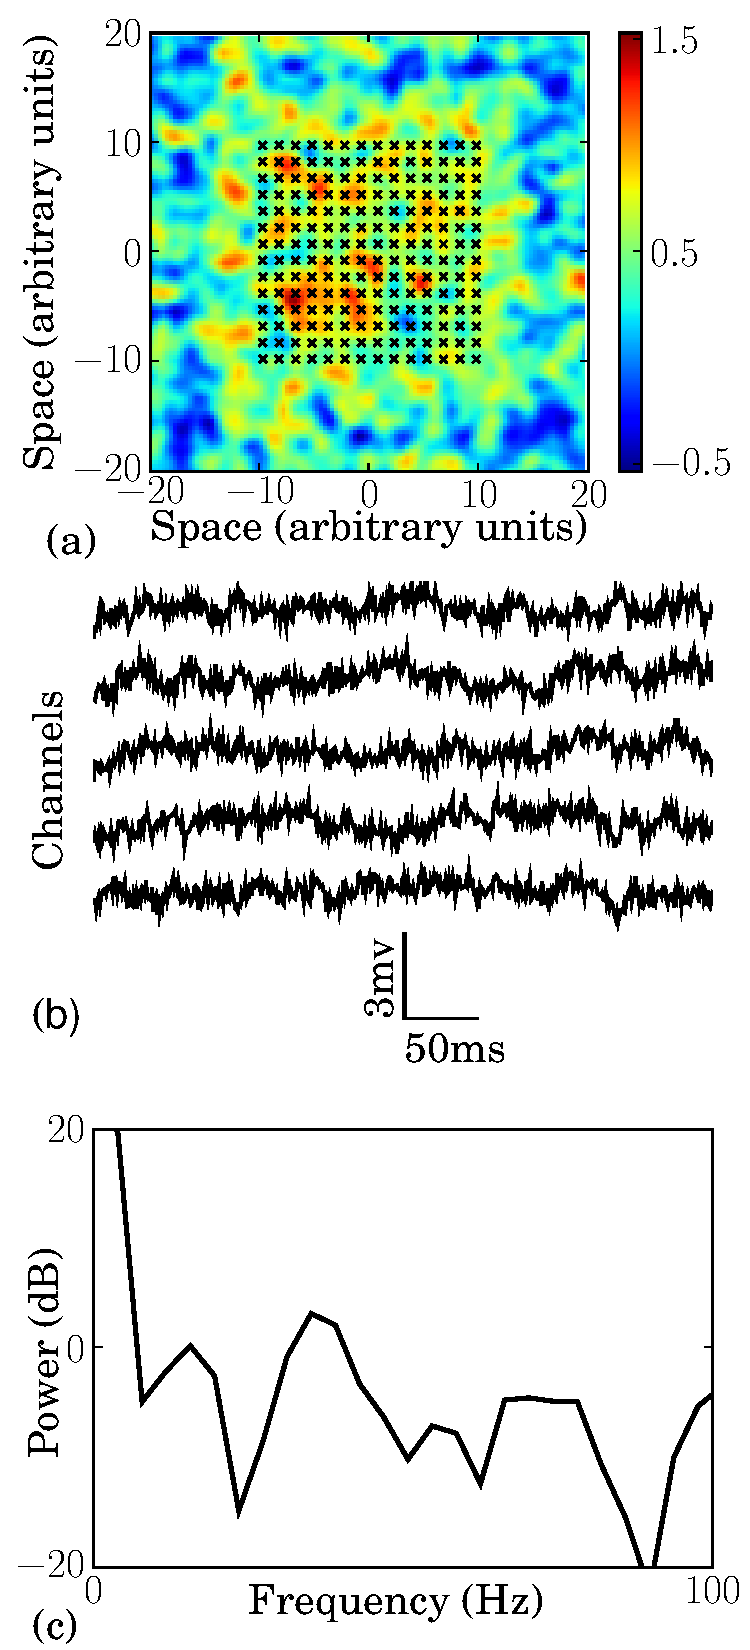
\includegraphics[width=0.3\textwidth]{./Graph/ExperimentFigurePy_1.pdf} 
   	\end{center}
   	\caption{Example of experimental design and model output. \textbf{a}. Example of the neural field with sensors. The centres of the sensors are shown by crossed and the sensor widths ($1/2$ height of Gaussian) are shown by the circles. \textbf{b} Example of data generated by the model through the observations. \textbf{c}. Power spectral density of the data generated by an observation showing the typical $1/f$ characteristic of iEEG.} 
   \end{figure}
% \begin{figure}[th]\label{fig:experimental design}
% \begin{center}
% \subfigure[][]{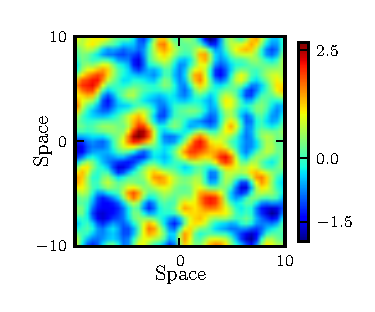
\includegraphics[width=0.35\textwidth]{./Graph/ExperimentFigurePy.pdf}}\\
% \subfigure[][]{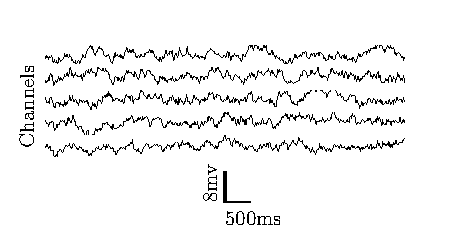
\includegraphics[width=0.35\textwidth]{./Graph/ExperimentFigureEEGPy.pdf}}\\
% \subfigure[][]{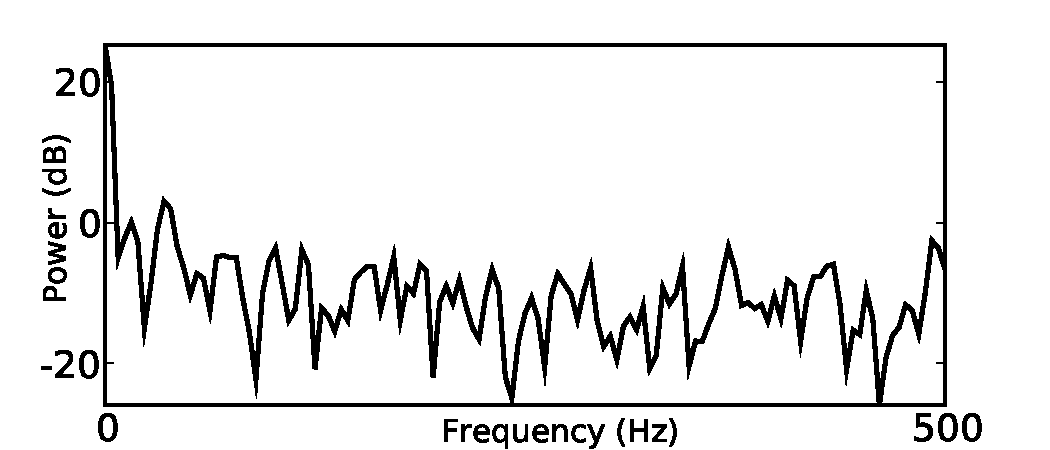
\includegraphics[width=0.35\textwidth]{./Graph/ExperimentFigurePSDPy.pdf}}
% \end{center}
% \caption{Example of experimental design and model output. \textbf{a}. Example of the neural field with sensors. The centres of the sensors are shown by crossed and the sensor widths ($1/2$ height of Gaussian) are shown by the circles. \textbf{b} Example of data generated by the model through the observations. \textbf{c}. Power spectral density of the data generated by an observation showing the typical $1/f$ characteristic of iEEG.} 
% \end{figure}
\begin{figure}[th]
\subfigure[][]{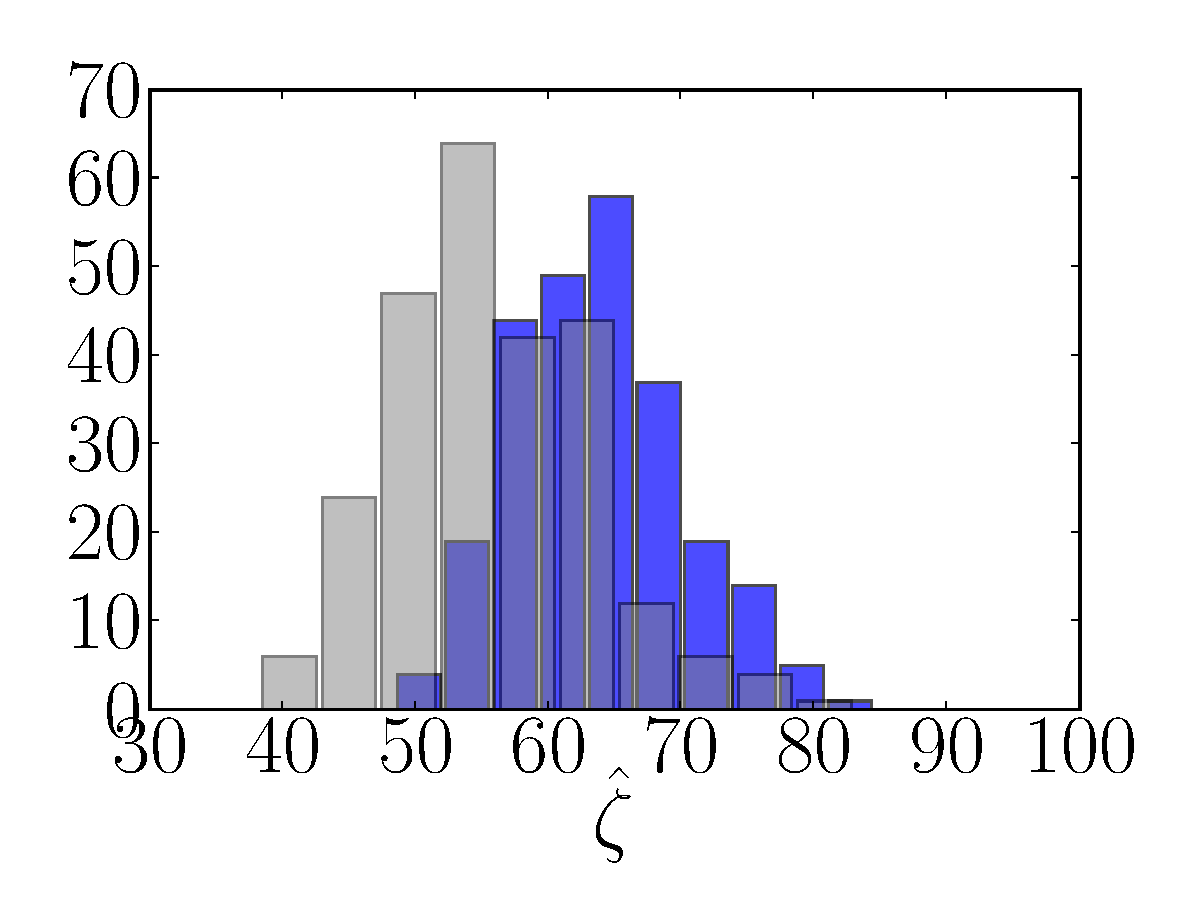
\includegraphics[width=0.24\textwidth]{./Graph/zeta.pdf}}
\subfigure[][]{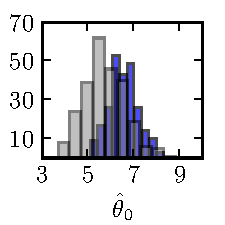
\includegraphics[width=0.24\textwidth]{./Graph/theta0.pdf}}\\
\subfigure[][]{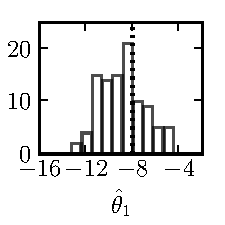
\includegraphics[width=0.24\textwidth]{./Graph/theta1.pdf}}
\subfigure[][]{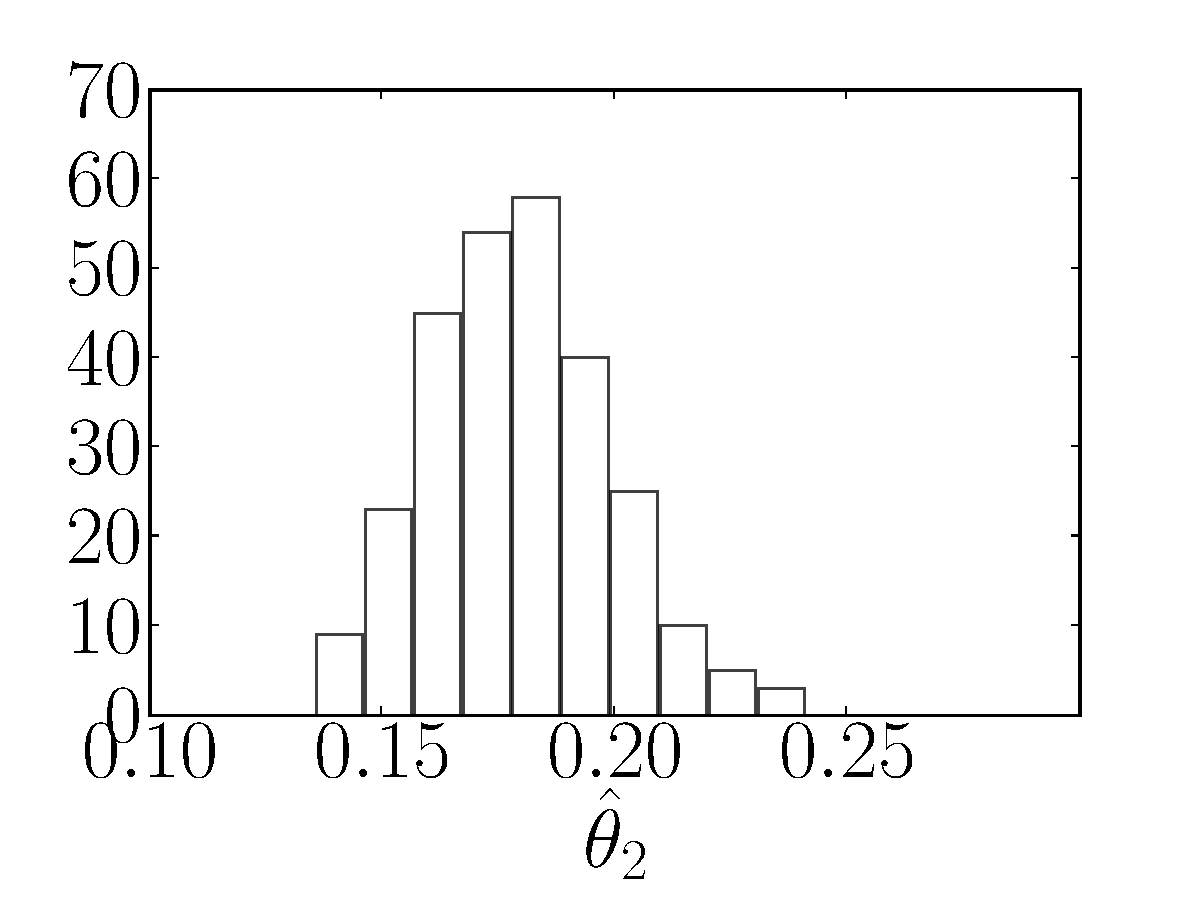
\includegraphics[width=0.24\textwidth]{./Graph/theta2.pdf}}
\caption{Distribution of the parameters estimates over 272
runs.}
\label{fig:Parameters}
\end{figure}
\subsection{Spatial Frequency Analysis} In accordance with Section~\ref{SpectralAnalysisSection}, the spatial frequency of the field was used to confirm the spacing and width of the sensors was adequate to capture the significant dynamics of the field. Figure~\ref{fig:FieldFFT} (part a.) shows the spatial frequency of the field. The cut-off frequency, $\nu_c$, was taken to be \omg{??} ($-3$~dB point). From equation~\ref{eq:MinimumSensorDistance}, this yielded a minimum sensor separation of \omg{??}. This confirms our separation of \omg{??} was enough to prevent problems associated with aliasing.

The spatial frequency of the observations is shown in Figure~\ref{fig:FreqAnalysis} (part c.). The peak power of the spatial frequency of the observations was approximately \omg{$??$}~dB. The cut-off frequency (-3~dB point) was taken to correspond to  approximately \omg{$??$}~dB. This provided a conservative estimate of the spatial bandwidth. The oversampling parameter $\rho_b$ was set to $??$ giving a minimum distance between basis functions of $??$ to satisfy Shannon's sampling criterion (from equation~\ref{eq:BasisFunctionSeparation}). \todo{maybe from Parham's derivation... From equation~\ref{} the width was calculated to be... or...}. The width of the basis functions was chosen such that they had sufficient overlap to represent the dynamic field.

\begin{figure*}
	\begin{center}
\subfigure[][]{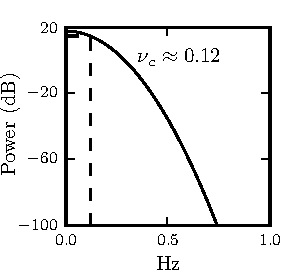
\includegraphics[width=0.3\textwidth]{./Graph/BasisChar.pdf}}
\subfigure[][]{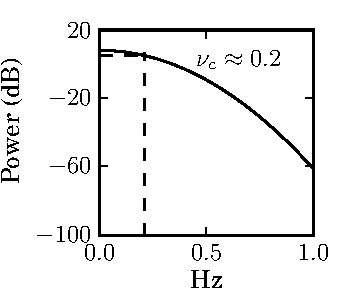
\includegraphics[width=0.3\textwidth]{./Graph/SensorChar.pdf}}
\subfigure[][]{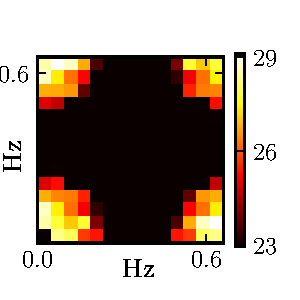
\includegraphics[width=0.3\textwidth]{./Graph/ObservationFrequencyResponse.pdf}}
	\end{center}
	\caption{a:Field basis function frequency response; b:Sensor frequency response ; c: The average FFT of the observed field.} 
\label{fig:FreqAnalysis} 
\end{figure*}
Following this, the distance between basis function, $\Delta_b$, was set to $2.5$ and the basis function width, $\sigma_{\phi}^2$, was set to 3.6, 3.16 mm full width at half maximum. Analysis said 3.9 from Parham's derivation, but 3.6 still overlaps and allows more high frequency details to be represented.

\subsection{State and Parameter Estimates} To demonstrate the performance of the parameter and state estimation, $200$ realisations of the data were generated. Each realisation consisted of 200~ms of data and the estimation was applied to the final 195~ms, allowing the model filter the initial conditions. The initial state and parameters were unknown to the estimator. The distribution of the parameters and the resulting kernel are shown in figure~\ref{fig:Parameters} and figure~\ref{fig:KernelEstimates} respectively. Although a wide distribution can be seen over the parameter estimates the ratio between them remans in a narrow range as shown in figure~\ref{fig:ParametersRatio}. The state estimates for one realization were evaluated by comparing the field reconstruction to the true field using the mean over time of the Root Mean Square Error (RMSE) and standard deviation of the RMSE giving $0.19\pm 0.01$. The RMSE of the field estimate over time is also shown in figure~\ref{fig:RMSE}. One snapshot for the original and the field estimate and their corresponding error are illustrated in figure~\ref{fig:FieldEstimate}.
\begin{figure}
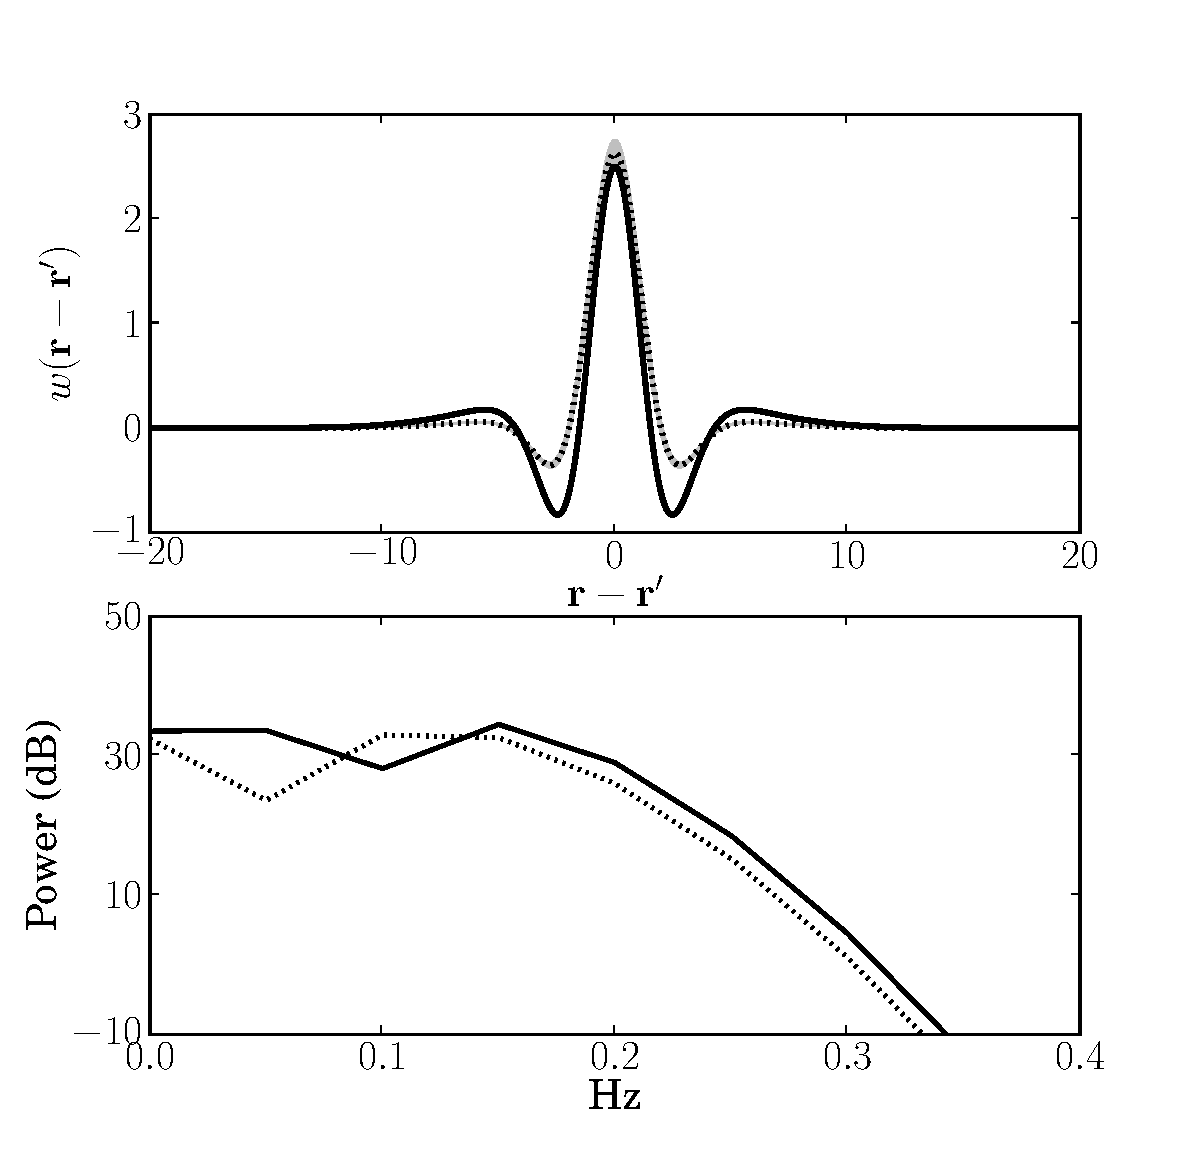
\includegraphics[width=0.5\textwidth]{./Graph/KernelEstimate_KernelFreqResponse.pdf}
\caption{Mean kernel estimates over 200 runs ;  true and estimated kernels are shown by solid
and dashed line respectively, the red area shows 95\% confedence interval; top: spatial domain; bottom: frequency domain}
\label{fig:KernelEstimates}
\end{figure}
\begin{figure}[th]
\subfigure[][]{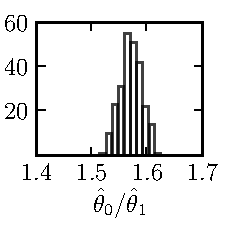
\includegraphics[width=0.24\textwidth]{./Graph/theta0_theta1_ratio.pdf}}
\subfigure[][]{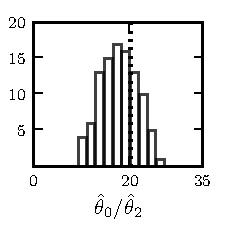
\includegraphics[width=0.24\textwidth]{./Graph/theta0_theta2_ratio.pdf}}\\
\caption{Distribution of the parameters ratios over 272 runs.}
\end{figure}
\label{fig:ParametersRatio}
\begin{figure}[th]
\subfigure[][]{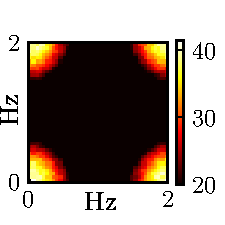
\includegraphics[width=0.24\textwidth]{./Graph/FFTTrueField.pdf}}\label{fig:FieldFFT}
\subfigure[][]{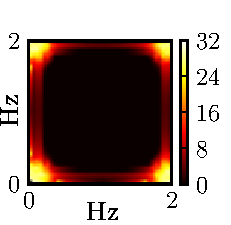
\includegraphics[width=0.24\textwidth]{./Graph/FFTEstimatedField.pdf}}\label{fig:EstimatedFieldFFT}\\
\caption{The average FFT of the hidden field; a: True field; b: Estimated field.}
\label{fig:FFTTrueEstimate}
\end{figure}

  \begin{figure}
   	\begin{center}
   		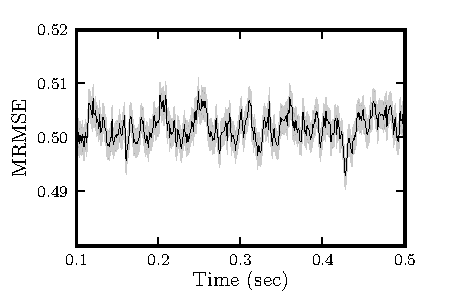
\includegraphics[width=0.5\textwidth]{./Graph/MRMSE.pdf} 
   	\end{center}
   	\caption{The RMSE of the estimated field over time.} 
\label{fig:RMSE}
   \end{figure}


\begin{figure*}[!th] 
\subfigure[][]{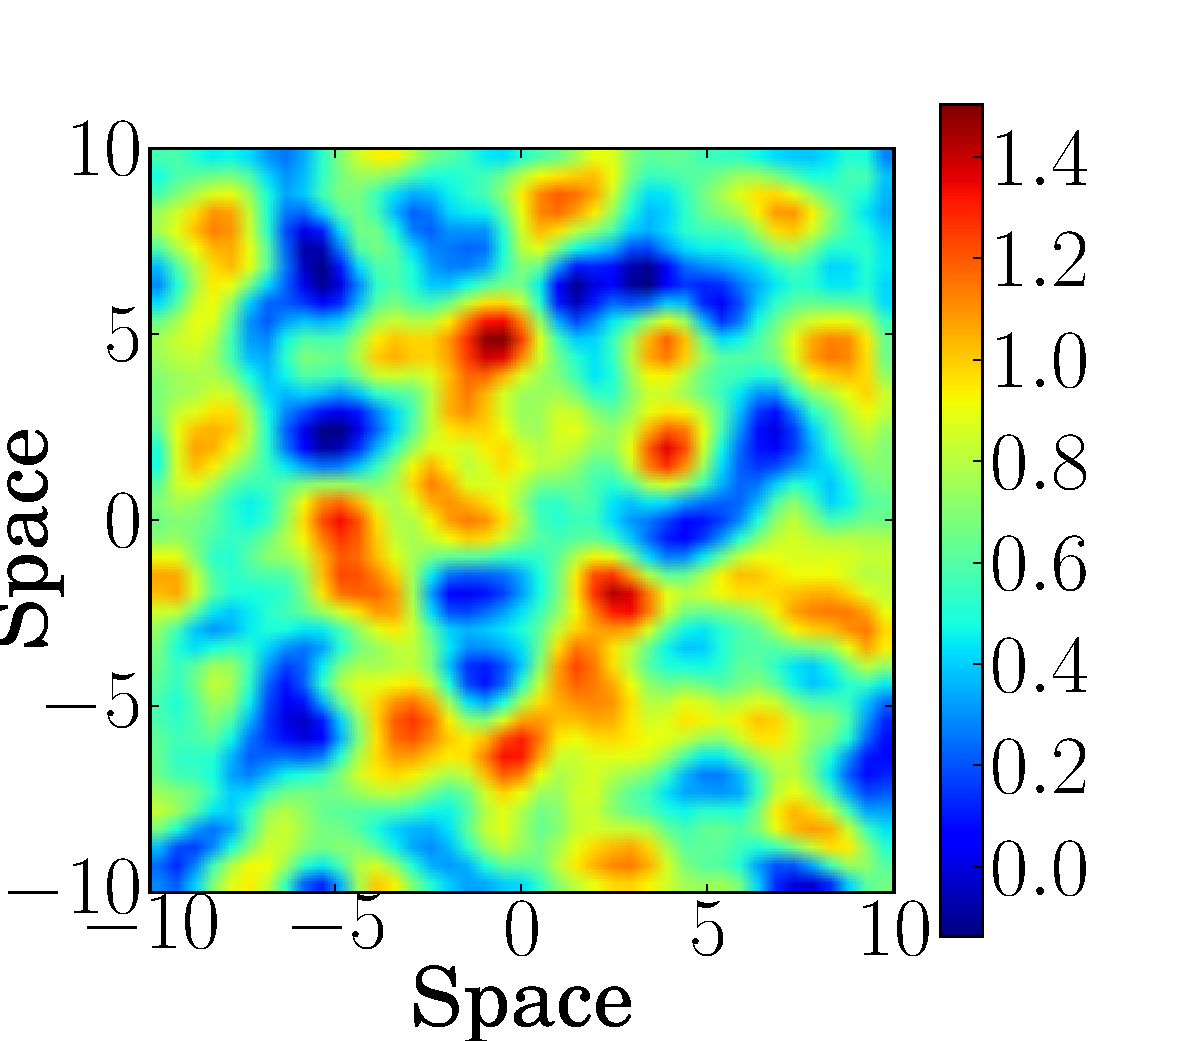
\includegraphics[width=2in]{./Graph/TrueField90.pdf}}
\subfigure[][]{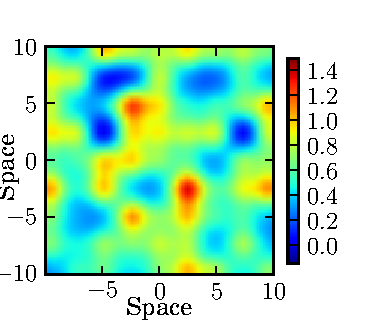
\includegraphics[width=2in]{./Graph/EstimatedField90.pdf}}
\subfigure[][]{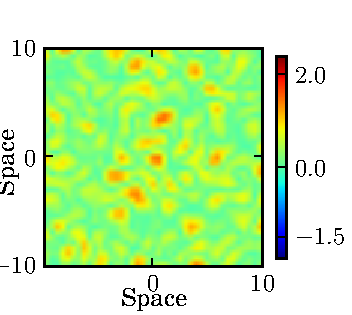
\includegraphics[width=2in]{./Graph/EstimationError90.pdf}}\\
\caption{One snapshot of the spatial field; a: True field; b: Estimated field; c: The absolute error.}
\label{fig:FieldEstimate}
\end{figure*}

\section{Discussion}\label{DiscussionSection}
This paper presents a novel framework for model reduction to facilitate practical state and parameter estimation of neural fields. The level of detail of the estimated field is related to the basis functions decomposition, thereby providing a flexible approach where a trade-off can be made between physiological detail and computational complexity. The choice of Gaussian basis functions can be justified by the existence of the so called bump solutions for this class of model~\cite{Coombes2005}. 

The frequency analysis and model selection tools presented in this paper specify the sensor and field basis function arrangement required to form a state-space model that is capable of capturing the dominant cortical dynamics. These tools can be also used to better design electrophysiological recording techniques to advance model-based neural parameter estimation in order to avoid spatial aliasing. The effect of the basis function decomposition will restrict the frequency content of the estimated field. This is evident in when comparing Figures~\ref{fig:FieldFFT} and~\ref{fig:EstimatedFieldFFT}. Since the frequency content of the field is governed by disturbance covariance and the shape of the connectivity kernel some information will be lost due the decomposition. The implication of this loss of information is the high spatial frequency content of the connectivity kernel. This is demonstrated in Figure~\ref{fig:KernelEstimates} of the results where the frequency content of the estimated connectivity kernel is less than the true kernel.

Even though the high frequency content of the connectivity kernel is lost though the basis function decomposition, the dominant dynamics are still captured with the estimated reduced model. This is illustrated in~\ref{fig:FieldEstimate}. In addition, the ratio of the kernel parameters falls into a tight distribution as seen in Figure~\ref{fig:ParametersRatio}. This indicates that the ratio of excitation to inhibition can be tracked with this approach. 

To the authors best knowledge, this is the first paper to propose an estimation framework for intracortical connectivity from electrophysiological data. The importance of this can be illustrated by considering the connectivity structure at this scale can not be estimated using diffusion tensor imaging due to the near isotropic diffusion or water in grey matter, the fine spatial scale and the high degree of crossing of fibres~\cite{Assaf2008}. In addition, other non-model based techniques for estimating functional connectivity such as Granger causality \cite{Hesse2003}, the direct transfer function \cite{Kaminski1991}, and partial directed coherence \cite{Sameshima1999} are restricted to the spatial scales of the recording electrodes. The model based technique proposed in this paper estimates the connectivity structure independently of the recording electrode geometry. An advantage of the auto-regressive (AR) based methods is that they allow for anisotropic connectivity, which is present in cortico-cortical fibres. The AR and the proposed model-based methods are complementary, where they estimating connectivity at different spatial scales. Therefore, by combining these methods a more realistic model can be estimated. A recent theoretical study~\cite{Jirsa2009} has demonstrated the importance of this multi-scale structure in generating the characteristic rhythms of the brain.

Generating patient specific neural field models has the potential to have significant impact on several areas of neuroscientific research and clinical neurology. Specifically, the development of a patient-specific state-space model will allow for the application of systems theoretical techniques from engineering to be applied to neuro-dynamics. For example, state tracking could be used in brain-computer interface or epileptic seizure prediction applications, where specific regions of the state-space may indicate intent of movement or imminent seizures. Recent studies using neural field models have demonstrated the theoretical implications of specific connectivity structure of the cortical columns in neural field models, where the connectivity kernel governs where a Turing-Hoft bifurcation occurs~\cite{Hutt2005}, and types of oscillations that can be generated~\cite{Schmidt2009}. This implies that if we could estimate the connectivity structure for an individual, then we could capture patient specific neurodynamics that lead to various oscillatory states. In addition, a patient specific state-space model will allow application of control engineering techniques to robustly prevent the neuro-dynamics entering pathological regions of state-space using electrical stimulation. 

Parameter estimation may have significant impact on the treatment of disease. For example, recent theoretical work has demonstrated that seemingly similar electrographic seizures in absence epilepsy may arise from abnormal excitatory or inhibitory mechanisms~\cite{Marten2009}. These very different mechanisms would require very different medications for successful treatment. However, the underlying mechanisms would be hidden from the clinician in the normal clinical setting. Successful parameter estimation has the potential to reveal these hidden mechanisms allowing for improved treatment strategies.

This estimation framework also has theoretical implications. This estimation framework has the potential to allow testing hypotheses that have been generated in theoretical studies and to validate neural field models. For example, it has been hypothesised that so called bump solutions are a possible mechanism for short term memory formation~\cite{Coombes2005}. Using the proposed model-based framework, we can reconstruct a neural field from data, and estimate parameters and check if they correspond the the theoretically derived parameters where these bump solutions can exist. In addition exploration of parameters and the state-space can be explored during other cognitive tasks and states of arousal such as sleep and anaesthesia. 

In this paper the widths of the connectivity kernel basis functions are assumed to be known. In a future work we plan to extend this work to unknown widths. We hope to achieve this by using a sufficiently large set of connectivity basis functions within the physiological plausible limits, and letting estimation procedure take care of the weights. In addition, the assumption homogeneity can be relaxed, where heterogeneity can be modelled by careful placement of field basis functions. For example, if cortical regions have a greater density of neural populations, then more basis functions can be used in these areas. In this scenario, model selection and basis function positioning can be achieved using instantaneous frequency analysis of the the neural field or alternative model selection tools based on information criteria.

\begin{itemize}
	\item What about the transient! The need for activity to perform estimation. \omg{To Learn You Must Perturb!} 
\end{itemize}

\section{Conclusion}\label{ConclusionSection}
\appendix 
\section{Discrete Time Model}\label{Time Discretization} To form the IDE neural field model a time discretization must be perform. We used a one-step Euler method where Eq.~\ref{FinalFormContinuous} can be approximated by 
\begin{eqnarray}
	\label{Euler Approximation} \lefteqn{\frac{v\left( \mathbf{r},t+T \right) - v\left( \mathbf{r},t\right)}{T_s} =}\nonumber\\
& -&\zeta v\left( \mathbf{r},t \right) + \int_\Omega {w\left( \mathbf{r}-\mathbf{r}' \right)f\left( {v\left( \mathbf{r}',t \right)} \right)d\mathbf{r}'}.\nonumber \\ 
\end{eqnarray}
For clarity, we shall index time points in the discrete time form of the model using the subscript $t$ and the next time point as $t+1$. Rearranging Eq.~\ref{Euler Approximation} we get 
\begin{eqnarray}
	\label{Euler Approximation2} v_{t+1}\left( \mathbf{r}\right) &=& v_t\left( \mathbf{r}\right) -T_s \zeta v_t\left( \mathbf{r}\right)\nonumber \\
&+& T_s \int_\Omega {w\left( \mathbf{r}-\mathbf{r}' \right)f\left( {v_t\left( \mathbf{r}'\right)} \right)d\mathbf{r}'}.\nonumber \\ 
\end{eqnarray}
The discrete time form of the model is 
\begin{equation}
	\label{Discrete Time Model1} v_{t+1}\left(\mathbf{r}\right) = \xi v_t\left(\mathbf{r}\right) + T_s \int_\Omega { w\left(\mathbf{r}-\mathbf{r}'\right) f\left(v_t\left(\mathbf{r}'\right)\right) d\mathbf{r}'}, 
\end{equation}
where $\xi = 1 - T_s \zeta$. 
\section{Numerical Simulation of IDE Model}\label{Space Discretization} To solve the intregro-difference equation in Eq.~\ref{Discrete Time Model1} we define the spatial aspect of the model on a regular square $i,j$ grid of neural masses, where the spatial step size $\Delta \mathbf{r}_i = \Delta \mathbf{r}_j = \Delta $ giving 
\begin{eqnarray}
	\label{discrete space} \lefteqn{v_{t+1}\left(\mathbf{r}_{ij}\right)=}\nonumber\\
&&\xi v_t\left(\mathbf{r}_{ij}\right)+T_s \Delta^2\sum_{i=1}^{i=I}{\sum_{j=1}^{j=J}{w\left(\mathbf{r}-\mathbf{r}_{ij}'\right)f\left( v_t\left( \mathbf{r}_{ij}'\right)\right)}}\nonumber\\
&+& e_t(\mathbf{r}_{i,j}), 
\end{eqnarray}
where $e_t(\mathbf{r}_{i,j}) \sim \mathcal{N}\left(0,\Sigma\right)$. We have used free boundary conditions and extended the spatial domain to alleviate problems associated with edge effects. 
\section{Reduction to Finite State-Space Model}\label{Simplifying Decomposition} Starting from Eq.~\ref{reduced continuous model} we multiply throughout by $\boldsymbol{\phi}(r)$ and integrate over the spatial domain $\Omega$ to get 
\begin{eqnarray}
	\label{StartofReduction}\lefteqn{ \int_\Omega {\boldsymbol{\phi} \left(\mathbf{r}\right)\boldsymbol{\phi}^{\top}\left(\mathbf{r}\right) d\mathbf{r}} \mathbf{x}_{t+1}=} \nonumber\\
 &&T_s \int_\Omega {\boldsymbol{\phi} (\mathbf{r}) \boldsymbol{\theta}^{\top} \int_\Omega {\boldsymbol{\psi} \left(\mathbf{r}-\mathbf{r}'\right) f\left(\boldsymbol{\phi}^{\top}\left(\mathbf{r}'\right) \mathbf{x}_t \right)d\mathbf{r}'}d\mathbf{r}} \nonumber\\
&-& \xi\int_\Omega {\boldsymbol{\phi}(\mathbf{r})\boldsymbol{\phi}^{\top}(\mathbf{r})d\mathbf{r}} \mathbf{x}_t+
\int_\Omega{\boldsymbol{\phi} \left(\mathbf{r}\right) e_t\left(\mathbf{r}\right)d\mathbf{r}}. 
\end{eqnarray}
Substituting equation~\ref{DefGamma} into equation~\ref{StartofReduction} and cross-multiplying by $\boldsymbol{\Gamma}^{-1}$ gives 
\begin{eqnarray}\label{eq:ReducedForm}
	 \lefteqn{\mathbf{x}_{t+1} \nonumber = T_s\boldsymbol{\Gamma}^{ - 1}\int_\Omega {\boldsymbol{\phi}(\mathbf{r}) \int_\Omega {f(\boldsymbol{\phi}^{\top}(\mathbf{r}')\mathbf{x}_t) \boldsymbol{\psi}^{\top} (\mathbf{r}-\mathbf{r}')d\mathbf{r}'} d\mathbf{r}} \boldsymbol{\theta}} \nonumber\\
&-&\xi\mathbf{x}_t + \boldsymbol{\Gamma}^{-1} \int_\Omega{\boldsymbol{\phi}(\mathbf{r})e_t(\mathbf{r})d\mathbf{r}}.\\ 
\end{eqnarray}
\section{}\label{ColoredNoise} 
\newtheorem{lemma}{Lemma} 
\begin{lemma}
	Consider the i.i.d. noise term $e_t\sim\mathcal{GP}(\mathbf 0,\gamma(\mathbf{s}-\mathbf{r}))$ then 
	\begin{equation}
		\mathbf e_t=\boldsymbol{\Gamma}^{-1}\int_\Omega {\boldsymbol{\phi} ( \mathbf{r} )e_t( \mathbf{r} )d\mathbf{r}} \label{eq:AppendixWt} 
	\end{equation}
	is a vector valued, zero mean normally distributed white noise process with covariance 
	\begin{equation}
		\boldsymbol\Sigma_e =\mathbf{\Gamma}^{-1}\int_{\Omega}\int_{\Omega}\boldsymbol{\phi}\left(\mathbf r\right) \gamma\left(\mathbf r- \mathbf r' \right)\boldsymbol{\phi}\left(\mathbf r'\right)^{\top}d\mathbf r' d\mathbf r\mathbf{\Gamma}^{- \top} 
	\end{equation}
	\label{lemma:FieldCovariance} 
\end{lemma}
\section*{Proof} Equation (\ref{eq:AppendixWt}) is a linear function of $e_t(\mathbf r)$ and hence $\mathbf{e}_t$ is also normally distributed. The expected value of $\mathbf e_t$ is given by 
\begin{eqnarray}
	\mathbf E\left[ \mathbf e_t\right]&=& \mathbf{\Gamma}^{-1}\int_{\Omega}\boldsymbol\phi\left(\mathbf{r}\right)\mathbf E\left[e_t\left(\mathbf{r}\right)\right] d\mathbf{r} \nonumber \\
	&=&\mathbf 0 
\end{eqnarray}
The covariance of $\mathbf{e}_t$ is 
\begin{eqnarray}
	\lefteqn{\mathbf{\Sigma}_e} \nonumber \\ 
&=&\mathbf{\Gamma}^{-1}\mathbf E[\int_{\Omega}\boldsymbol{\phi}(\mathbf{r})e_t(\mathbf{r})d\mathbf{r} \int_{\Omega}\boldsymbol{\phi}^{\top}(\mathbf{r}') e_t(\mathbf{r}')d\mathbf{r}']\mathbf{\Gamma}^{- \top} \nonumber \\
	&=&\mathbf{\Gamma}^{-1}\int_{\Omega}\int_{\Omega} \boldsymbol{\phi}(\mathbf{r}) \mathbf E[e_t(\mathbf{r})e_t(\mathbf{r}')]\boldsymbol{\phi}^{\top}(\mathbf{r}')d\mathbf{r}' d\mathbf r\mathbf{\Gamma}^{- \top} \nonumber\\
	&=&\mathbf{\Gamma}^{-1}\int_{\Omega}\int_{\Omega}\boldsymbol{\phi}(\mathbf r) \gamma(\mathbf r- \mathbf r' )\boldsymbol{\phi}^{\top}(\mathbf r')d\mathbf r' d\mathbf r\mathbf{\Gamma}^{-\top} 
\end{eqnarray}
\section{Proof of \ref{eq:GaussianFT} and \ref{eq:WidthFrequencyRelationship} }\label{ap:FrequencyAnalysis}
Applying the \textit{n}-dimensional Fourier transform \cite{Arsac1966} to an \textit{n}-dimensional Gaussian centered at the origin yields
\begin{eqnarray}\label{eq:AppendixGaussianFT}
 \lefteqn{\boldsymbol\Phi(\boldsymbol \nu)=\int_{\mathcal R^n}\mathrm{exp}({-\frac{1}{\sigma_{\phi}^2}\mathbf r^\top\mathbf r})\mathrm{exp}(-2\pi i\boldsymbol\nu^\top\mathbf r)d\mathbf r} \nonumber \\
&=&\int_{\mathcal R^n}\mathrm{exp}(-\frac{1}{\sigma_{\phi}^2}\left[\mathbf r +\sigma_{\phi}\pi i \boldsymbol\nu\right]^\top\left[\mathbf r +\sigma_{\phi}\pi i \boldsymbol\nu\right])d\mathbf r \nonumber \\
&\times& \mathrm{exp}(-\sigma_{\phi}^2\pi^2\boldsymbol\nu^\top \boldsymbol\nu)
\end{eqnarray}
where 
\begin{eqnarray}\label{eq:IntegralOfGaussian}
\int_{\mathcal R^n}\mathrm{exp}(-\frac{1}{\sigma_{\phi}^2}\left[\mathbf r +\sigma_{\phi}\pi i \boldsymbol\nu\right]^\top\left[\mathbf r +\sigma_{\phi}\pi i \boldsymbol\nu\right])d\mathbf r&& \nonumber \\
=(\pi\sigma_{\phi}^2)^{\frac{n}{2}}&&
\end{eqnarray}
substituting \ref{eq:IntegralOfGaussian} in \ref{eq:AppendixGaussianFT} gives another scaled  Gaussian 
\begin{equation}
   \boldsymbol\Phi(\boldsymbol\nu)=(\pi\sigma_{\phi}^2)^{\frac{n}{2}}\mathrm{exp}(-\sigma_{\phi}^2\pi^2\boldsymbol\nu^\top \boldsymbol\nu)
\end{equation}
substituting $\sigma_{\nu}^2=\frac{1}{\pi^2\sigma_{\phi}^2}$ gives 
\begin{equation}
\boldsymbol\Phi(\boldsymbol \nu)=(\frac{1}{\pi\sigma_{\nu}^2})^{\frac{n}{2}}\mathrm{exp}(-\frac{1}{\sigma_{\nu}^2}\boldsymbol\nu^\top \boldsymbol\nu).
\end{equation}
and hence completing the proof. For 3 dB attenuation at $\boldsymbol\nu_c$ we need to set
\begin{eqnarray}
 |\boldsymbol\Phi(\boldsymbol\nu_c)|^2=\frac{1}{2}|\boldsymbol\Phi(\mathbf 0)|^2
\end{eqnarray}
%\left(\frac{1}{\pi\sigma_{\nu}^2}\right)^{n}\mathrm{exp}\left(-\frac{2}{\sigma_{\nu}^2}\boldsymbol\nu_c^\top \boldsymbol\nu_c\right)\\
solving for $\sigma_{\nu}^2$ we get
\begin{equation}
 \sigma_{\nu}^2=\frac{2\boldsymbol\nu_c^\top \boldsymbol\nu_c}{\ln 2 }.
\end{equation}

\section{Parameter Estimation Using Least Squares}\label{LeastSquaresAppendix} 
The finite state space model  given in \ref{eq:ReducedForm} is linear in parameters and therefore Least Square (LS) method can be applied to estimate the unknown parameters. We define $n_x \times n_{\theta}$ matrix
\begin{eqnarray}\label{eq:QMatrix}
	\lefteqn {\mathbf{Q}(\mathbf{x}_t)=} \\
&&\boldsymbol{\Gamma}^{ - 1}\int_\Omega {\boldsymbol{\phi}(\mathbf{r}) \int_\Omega {f(\boldsymbol{\phi}^{\top}(\mathbf{r}')\mathbf{x}_t)\boldsymbol{\psi}^{\top} \left(\mathbf{r}-\mathbf{r}'\right)d\mathbf{r}'} d\mathbf{r}}\nonumber
\end{eqnarray}
by substituting \ref{eq:Reducednoiseterm} and \ref{eq:QMatrix} in \ref{eq:ReducedForm} with zero input and using $\xi = 1-\zeta T_s$ at each time instant we can write
\begin{eqnarray}
	\mathbf x_{1}&=&\mathbf x_{0}+T_s \mathbf Q(\mathbf x_0) \boldsymbol{\theta}-\zeta T_s\mathbf x_0+\mathbf e_0 \nonumber \\
	\mathbf x_{2}&=&\mathbf x_{1}+T_s \mathbf Q(\mathbf x_1) \boldsymbol{\theta}-\zeta T_s\mathbf x_1+\mathbf e_1\nonumber\\
	&\vdots& \\
	\mathbf x_{n}&=&\mathbf x_{n-1}+T_s \mathbf Q(\mathbf x_{n-1}) \boldsymbol{\theta}-\zeta T_s\mathbf x_{n-1}+\mathbf e_{n-1} \nonumber
\end{eqnarray}
% in matrix form 
% \begin{equation}
% 	\left[
% 	\begin{array}{cccc}
% 		\mathbf x_{1}\\\mathbf x_{2}\\\vdots\\\mathbf x_{n}
% 	\end{array}
% 	\right] -\left[
% 	\begin{array}{cccc}
% 		\mathbf x_{0}\\\mathbf x_{1}\\\vdots\\\mathbf x_{n-1}
% 	\end{array}
% 	\right] =T_s\left[
% 	\begin{array}{cc}
% 		\mathbf Q(\mathbf x_0)&-\mathbf x_{0}\\\mathbf Q(\mathbf x_1)&-\mathbf x_{1}\\\vdots\\
% 		\mathbf Q(\mathbf x_{n-1})&-\mathbf x_{n-1}
% 	\end{array}
% 	\right] \left[
% 	\begin{array}{cc}
% 		\boldsymbol{\theta} \\
% 		\zeta
% 	\end{array}
% 	\right]+\left[
% 	\begin{array}{cccc}
% 		\mathbf e_0\\\mathbf e_1\\\vdots\\\mathbf e_{n-1}
% 	\end{array}
% 	\right] 
% \end{equation}
 in compact form we have 
\begin{equation}
	\mathbf Z=\mathbf X \mathbf W+\boldsymbol \xi 
\end{equation}
where 
\begin{small}
\begin{equation*}
	\mathbf Z=\left[
	\begin{array}{cccc}
		\mathbf x_{1}-\mathbf x_{0}\\
		\mathbf x_{2}-\mathbf x_{1}\\\vdots\\
		\mathbf x_{n}-\mathbf x_{n-1}
	\end{array}
	\right],\quad \mathbf X=T_s\left[
	\begin{array}{cccc}
		\mathbf Q(\mathbf x_0)&-\mathbf x_{0}\\
		\mathbf Q(\mathbf x_1)&-\mathbf x_{1}\\\vdots\\
		\mathbf Q(\mathbf x_{n-1})&-\mathbf x_{n-1}
	\end{array}
	\right] 
\end{equation*}
\end{small}
and
\begin{small}
\begin{equation*}
\quad \mathbf W=\left[
	\begin{array}{cc}
		\boldsymbol{\theta} \\
		\zeta
	\end{array}
	\right],\quad \boldsymbol \xi=\left[
	\begin{array}{cccc}
		\mathbf e_0\\\mathbf e_1\\\vdots\\\mathbf e_{n-1}
	\end{array}
	\right] 
\end{equation*}
\end{small}
using the LS method $ \mathbf W$ can be estimated 
\begin{equation}
	\mathbf W\approx(\mathbf X^\top\mathbf X)^{-1}\mathbf X^\top\mathbf Z 
\end{equation}
\section{Parameters} 
\begin{tabular}
	{c|c} Symbol & Description \\
	\hline
	\\ & \textbf{Domain and indicies} \\
	\hline
	$\Omega$ & spatial domain \\
	$t$ & time (seconds) \\
	$\mathbf{r}$ & spatial location \\
	$n$ & sensor index $n=1,..,N$ \\
	$T$ & time step \\
	\\ & \textbf{Spatiotemporal Signals} \\
	\hline
	$y(\mathbf{r}_n,t)$ & observation \\
	$v(\mathbf{r},t)$ & mean membrane potential \\
	$g(\mathbf{r},t)$ & average action potential rate \\
	$f(\mathbf{r},t)$ & firing function rate \\
	$u(\mathbf{r},t)$ & external input \\
	$e(\mathbf{r},t)$ & field disturbance, covariance $\gamma$\\
	$\epsilon(\mathbf{r}_n,t)$ & observation noise, covariance $\Sigma_\epsilon$ \\
	\\ & \textbf{Model} \\
	\hline
	$h(t)$ & post-synaptic response kernel \\
	$m(\mathbf{r},\mathbf{r}')$ & sensor kernel, variance $\sigma_m^2$ \\
	$\eta(t)$ & Heaviside function \\
	$\zeta$ & inverse synaptic time constant \\
	$w(\mathbf{r},\mathbf{r}')$ & spatial connectivity kernel \\
	$f_{max}$ & maximal firing rate \\
	$\varsigma$ & slope of sigmoidal activation function \\
	$v_0$ & firing threshold \\
	$\delta(t)$ & Dirac-delta function \\
	$D$ & Temporal differential operator \\
	$\xi$ & time constant parameter \\
	\\ & \textbf{Decomposition} \\
	\hline
	$L$ & number of field basis functions  \\
	$\mathbf{\phi(r)}$ & vector of Gaussian basis functions \\
	$\mathbf{x}_t$ & state vector at time $t$ \\
	$\mathbf{\psi}$ & vector of connectivity kernel basis functions \\
	$\theta$ & vector of connectivity kernel parameters \\
	$\Gamma$ & inner product of field basis functions \\
	$q()$ & state function \\
	$k()$ & maps into to discrete state of input function \\
	$\mathbf{e}_t$ & state disturbance, covariance $\Sigma_e$ \\
	$\mathbf{C}$ & observation matrix \\
	\\ & \textbf{Frequency Analysis} \\
	\hline
	$V(\nu)$ & Spectrum of the dynamic field \\
	$\nu$ & Spatial frequency \\
	$\nu_c$ & Spatial cut-off frequency \\
	$\Delta_s$ & Distance between adjacent sensors \\
	$\rho$ & Over-sampling parameter \\
	$\Delta_b$ & Distance between field basis functions \\
	$\sigma_{nu}^2$ & Variance of FT of Gaussian basis function \\
	$\sigma^2$ & Spatial variance of Gaussian in spatial domain \\
	\\ & \textbf{State Estimation} \\
	\hline
	$\hat{\mathbf{x}}$ & State estimate \\
	$\chi$ & Matrix of sigma vectors \\
	$\hat{\mathbf{x}}_t^{f-}$ & Forward prior estimate \\
	$\hat{\mathbf{x}}_t^f$ & Forward posterior estimate \\
	$\hat{\mathbf{x}}_t^{b-}$ & Backward prior estimate \\
	$\hat{\mathbf{x}}_t^{b}$ & Backward posterior estimate \\
	$P^f_t$ & Forward posterior covariance matrix \\
	$P^{f-}_t$ & Forward prior covariance matrix \\
\end{tabular}
\section*{References} 
\bibliographystyle{unsrt} 
\bibliography{BrainIDE}

% \begin{thebibliography}{10}
% \bibitem{book1} Goosens M, Rahtz S and Mittelbach F 1997 {\it The \LaTeX\ Graphics Companion\/} 
% (Reading, MA: Addison-Wesley)
% \bibitem{eps} Reckdahl K 1997 {\it Using Imported Graphics in \LaTeX\ } (search CTAN for the file `epslatex.pdf')
% \end{thebibliography}
\end{document}
